\documentclass[UTF8, twocolumn]{ctexart}
\usepackage{geometry}
\usepackage{graphicx}
\usepackage{float}

\CTEXsetup[format={\Large\bfseries}]{section}

\geometry{
  a4paper,
  top = 20mm,
  bottom = 20mm,
  left = 20mm,
  right = 20mm
}

\pagestyle{plain}

\title{案例学习:素描模拟绘制方法}
\author{张家侨 \and 张涵玮 \and 张骏 \and 张彬熠 \and 张漫榕 \and 袁均良}

\begin{document}

  \maketitle

  \section{引言}
    图像模拟绘制是数字图像处理领域重要的研究方向之一,许多科研工作者在这个方向发表过大量的论文。
    图像模拟绘制包括对各种艺术绘画的重现,即将一张真实自然图片模拟为油画、铅笔素描、彩色素描等
    绘画图像。
    \par
    在艺术绘画中,素描绘画是普遍性较强,被广泛学习的一种绘画方法。
    本案例学习以潘、纪、陈等人\cite{ji}的彩色素描模拟方法为案例,学习其中的原理,
    并实现基于线积分卷积的彩色铅笔素描模拟绘制方法。

  \section{彩色铅笔素描绘制流程}

    \subsection{总体流程}
    根据真实图像生成一张铅笔素描模拟图,属于底层图像处理,即输入与输出都是数字图像。根据
    \cite{ji}的方法,一张素描模拟图由三张图叠加而成,分别是颜色图、纹理图和轮廓图。
    颜色图由K-means聚类算法\cite{kmeans}和双色调映射方法\cite{duotones}结合产生;纹理图
    由3部分叠加而成,分别是线积分卷积方法\cite{lic}产生的卷积纹理图、纸肌理图和噪声图;
    轮廓图则通过霓虹变换\cite{outline}的方法产生。

    \subsection{生成颜色图}
    颜色图的生成属于图像预处理。对于一般的自然图像而言,其颜色丰富程度极高,颜色渐变性很强,而
    彩色素描图由若干个有限的颜色绘制而成,丰富程度较为有限,因此应当将原图的颜色丰富程度
    以及分布规律向彩色素描图的方向靠拢。原文采用的是K-means聚类算法\cite{kmeans}和双色调
    映射\cite{duotones}相结合的方法生成颜色图,即现将原图进行K-means图像聚类分割,然后通过
    双色掉映射的方法赋予每一个聚类主色调和副色调,最后进行两种颜色的融合。

      \subsubsection{K-means聚类分割}
      使用K-means聚类分割算法,将原始图像的像素点分类,每一类单独赋予一种颜色。K值的确定可以
      手工赋值,也可以根据图像的颜色丰富度计算得到。颜色丰富度的计算主要是通过计算图像在
      HSV色彩控件的Hue色调直方图确定。

      \subsubsection{基于双色调映射的颜色计算}
      原文中先确定一个基本颜色库,共有12种颜色,计算每个颜色到聚类中心的欧式距离,取距离最小的
      颜色作为该聚类的主色调。并通过双色调映射的方法计算出该聚类的副色调,具体方式是:将颜色
      转化到XYZ色彩控件,计算另外是一种颜色的映射结果色,取与聚类中心距离最小的颜色作为
      该聚类的副色调。主副色调计算完成之后,再通过双色调映射的方法融合并作为该聚类的颜色。

      \subsubsection{实现}
      双色调映射的方法是一种颜色重绘的方法,
      但是在实际情况中,发现这样做的效果并不能很好地模拟素描图像的颜色,
      在一些情况下颜色会产生较大的偏差,
      从图\ref{fig:artresult}可见,苹果的颜色甚至变为了黄褐色,显然不是想要的结果。
      \begin{figure}[htbp]
        \begin{center}
          \includegraphics[width=8cm]{../assets/artresult.png}
          \caption{原文比较结果,最右为原文实现}
          \label{fig:artresult}
        \end{center}
      \end{figure}
      \par
      经过分析,主要有两方面的原因,第一,K-means聚类算法的聚类中心可能并不适合作为该区域颜色
      的代表,尤其是当K值较小时;第二,由于基本颜色库的颜色数目较少,并不适合对原图进行大量的
      聚类,导致原图许多复杂的颜色区域可能被归为同一类,使得所求颜色被不合理地混合,从而产生
      错误的颜色。
      \begin{figure}[htbp]
        \begin{center}
          \includegraphics[width=8cm]{../assets/basecolorlib.png}
          \caption{原文的基本颜色库}
          \label{fig:basecolorlib}
        \end{center}
      \end{figure}
      综上所述,根据我们小组当前掌握的知识,难以完美重绘产生彩色素描图像相应的颜色,因此在实现
      中直接采用原图作为颜色图;从艺术的角度来说,这样产生的素描图相当于一张艺术大师绘制的
      图像,相较于一般的素描图来说略微有一些不真实。是一个较为折中的解决办法。

    \subsection{生成纹理图}
      纹理图是本案例生成素描图像的重点部分,纹理图的质量直接决定了生成结果的模拟相似程度。这一
      部分原文的方法是比较合理的,产生的纹理图效果较好。
      \subsubsection{生成噪声图}
        噪声图的叠加是为了模拟铅笔碳粒的颗粒感,同时实际铅笔绘画中铅笔是有轻重变化的,因此生
        成的噪声图必须有梯度和层次,不能完全使用二值图作为噪声图。采用原文的公式,将0到255的
        灰度值分成3个不同的范围,添加一定的随机变量,使得噪声图的层次感更强,明暗变化更明显。
        采用MATLAB实现的噪声图如图\ref{fig:noise}所示。
        \begin{figure}[htbp]
          \begin{center}
            \includegraphics[width=8cm]{../assets/noise.png}
            \caption{噪声图}
            \label{fig:noise}
          \end{center}
        \end{figure}
      \subsubsection{生成卷积纹理图}
        采用线积分卷积\cite{lic}的方法对噪声图进行卷积生成纹理图,
        其原理是因为黑白噪声图结合方向矢量场进行
        卷积的结果与手绘的铅笔素描纹理非常类似。采用MATLAB实现的纹理图如图\ref{fig:lic}
        所示。
        \begin{figure}[htbp]
          \begin{center}
            \includegraphics[width=8cm]{../assets/lic.png}
            \caption{纹理图、噪声图、纸肌理三者叠加后的结果}
            \label{fig:lic}
          \end{center}
        \end{figure}
      \subsubsection{叠加纸肌理}
        纸肌理的叠加主要是为了模拟在不同画材上绘制铅笔画的材质感,主要考虑要素是纸材质平面的
        凸起和凹陷,原文将其作为高度场考虑,但是实际上纸肌理对图像的作用较小,起到一个
        细节修饰的作用。图\ref{fig:lic}是已经叠加完成了纸肌理的纹理图像。
        \par
        将三者叠加起来的效果如图\ref{fig:lic}所示。

    \subsection{生成轮廓图}
      轮廓是素描绘画的重要组成部分之一,原文采用的霓虹变换\cite{outline}的方法是一种效果
      较好的方法,能够生成连续、精致的边缘,并且没有多余信息,采用原文方式产生的轮廓图如
      图\ref{fig:outline}所示。
      \begin{figure}[htbp]
        \begin{center}
          \includegraphics[width=8cm]{../assets/outline.png}
          \caption{轮廓图}
          \label{fig:outline}
        \end{center}
      \end{figure}

    \section{实现结果}
      走完上述流程之后,即可生成一张完整的彩色铅笔素描图像,为了体现卷积纹理的效果,也做了灰度
      图像的铅笔素描图像生成,实现的结果如图\ref{fig:result}所示。
      \begin{figure}[H]
        \begin{center}
          \begin{tabular}{c}

            \begin{minipage}{0.33\hsize}
              \begin{center}
                \includegraphics[width=3cm]{../assets/lenna_origin.png} \\
                \includegraphics[width=3cm]{../assets/building_origin.png} \\
                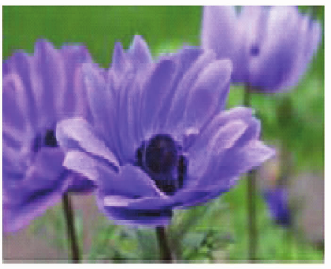
\includegraphics[width=3cm]{../assets/test1.png} \\
                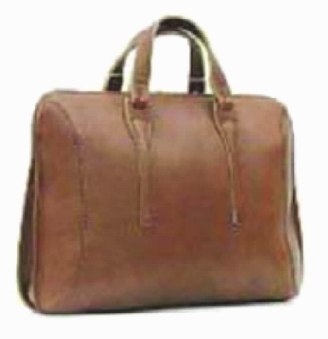
\includegraphics[width=3cm]{../assets/test2.png} \\
                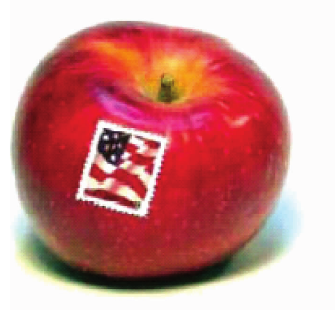
\includegraphics[width=3cm]{../assets/test3.png} \\
                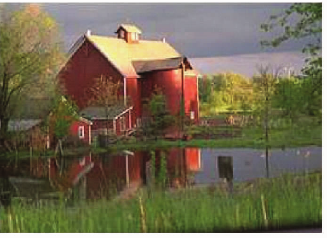
\includegraphics[width=3cm]{../assets/test4.png} \\
                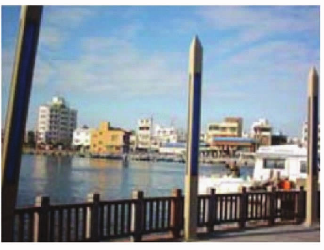
\includegraphics[width=3cm]{../assets/test5.png} \\
                原图
              \end{center}
            \end{minipage}

            \begin{minipage}{0.33\hsize}
              \begin{center}
                \includegraphics[width=3cm]{../assets/lenna_gray_result.png} \\
                \includegraphics[width=3cm]{../assets/building_gray_result.png} \\
                \includegraphics[width=3cm]{../assets/test1_gray_result.png} \\
                \includegraphics[width=3cm]{../assets/test2_gray_result.png} \\
                \includegraphics[width=3cm]{../assets/test3_gray_result.png} \\
                \includegraphics[width=3cm]{../assets/test4_gray_result.png} \\
                \includegraphics[width=3cm]{../assets/test5_gray_result.png} \\
                铅笔素描结果
              \end{center}
            \end{minipage}

            \begin{minipage}{0.33\hsize}
              \begin{center}
                \includegraphics[width=3cm]{../assets/lenna_result.png} \\
                \includegraphics[width=3cm]{../assets/building_result.png} \\
                \includegraphics[width=3cm]{../assets/test1_result.png} \\
                \includegraphics[width=3cm]{../assets/test2_result.png} \\
                \includegraphics[width=3cm]{../assets/test3_result.png} \\
                \includegraphics[width=3cm]{../assets/test4_result.png} \\
                \includegraphics[width=3cm]{../assets/test5_result.png} \\
                彩色素描结果
              \end{center}
            \end{minipage}

          \end{tabular}
          \caption{实现结果}
          \label{fig:result}
        \end{center}
      \end{figure}






  \begin{thebibliography}{9}
    \bibitem{ji} 潘龙, 纪庆革, 陈靖.
      ``线积分卷积与双色调映射相结合的彩色素描模拟方法'',
      {\sl 中国图像图形学报}, vol. 22, p875-885, 2017.
    \bibitem{kmeans} Burney S M A, Tariq H.
      ``K-means cluster analysis for image segmentation[J],''
      in {\sl International Journal of Computer Application},
      2014, 96(4): 1-8. [ DOI: 10.5120/16779-6360 ]
    \bibitem{duotones} Power J. L., West B. S., Stollnitz E. J., et al.
      ``Reproducing color images as duotones[C],''
      in {\sl Proceedings of the 23rd Annual Conference on Computer Graphics
      and Interactive Techniques}, New York: ACM, p237-248, 1996.
    \bibitem{lic} Cabral B., Leedom L. C..
      ``Imaging vector fields using line integral convolution[C]''
      in {\sl Proceedings of the 20th Annual Conference on Computer Graphics
      and Interactive Techniques}, New York: ACM, p263-270, 1993.
    \bibitem{outline} 李龙生, 周经野, 陈益强, 等.
      ``一种改进的铅笔画的生成方法[J],''
      {\sl 中国图像图形学报}, vol. 12, p1423-1429, 2007.
  \end{thebibliography}

\end{document}
